%
%     巻頭言
%

\documentclass[10pt,b5paper,papersize,dvipdfmx]{jsbook}

\usepackage{vuccaken}
\usepackage{vuccaken2019}

% --------------------------------------
\begin{document}

\begin{preface}{巻頭言}
        {機械工学科2回生}
        {\vname{西條}{晴幸}}
        {令和元年11月27日}
  %%
  物理科学研究会会長の西條晴幸です。今年度は令和最初の年であり、時代が節目を迎える年ですね。そんな中弊物理科学研究会も二つの意味で節目を迎えていました。ひとつは弊研究会の全身である核物理研究会の1949年発足から数えて70周年を迎えること、もうひとつはここ2年間で新入部員が一人のみといういよいよ廃部の危機的な意味で、です。今年部員が入らなければ本当にいや、危なかった...ここで登場するのが敏腕新歓担当さいj嘘ですひとえに前会長,前々会長による物理科学科新入生への積極的な働きかけにより、5人もの新入部員を迎え入れることができました。歴史的に見てもここ数年で70周年を迎える学友会諸団体は多く、それらと肩を並べてここまで弊研が続いて来られたのは先輩方の途切れることのない活動のためです。この70というひとつの節目を、これからの存続を感じさせる状態(部員獲得)で迎えられたことは非常に喜ばしいと感じています。\par
  ほげぇほげぇ
\end{preface}


%%
\clearpage
\quad\vfill
\begin{figure}[htb]
  \centering
  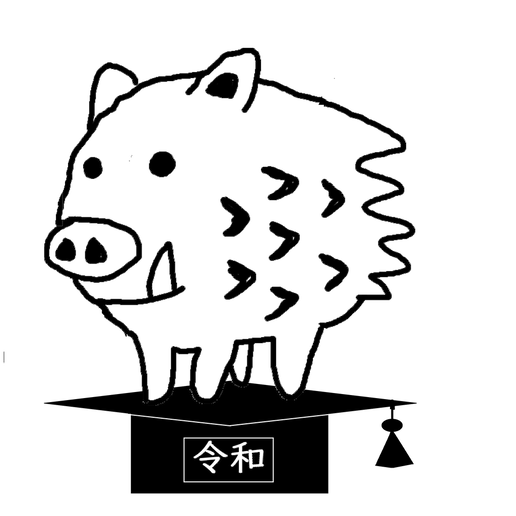
\includegraphics[width=40mm]{img/inoshishi.png}
  \caption*{
    \setlength{\baselineskip}{1.2zw}\gtfamily
    ボツ表紙 \\ 作・西村宗悟
  }
  \label{}
\end{figure}
\vfill

\end{document}
%
% お疲れさまです
%